% Дуников Константин Артёмович 

% Тип документа: статья, на бумаге А4
\documentclass[a4paper]{article}

% Подключение сторонних tex файлов 
\usepackage{import}


% Основные данные - ВУЗ, факультет, город...
\import{./../../stuff/tex}{config.tex}
% Небольшой набор инструментов
\import{./../../stuff/tex}{tools.tex}

% Подключение необходимых зависимостей
\import{./../../stuff/tex/settings}{packages.tex}
% Настройка подключенных пакетов
\import{./../../stuff/tex/settings}{preferences.tex}


% Шаблон титульной страницы 
\import{./../../stuff/tex/templates}{title.tex}
% Упрощенный блок "выполнил"
\import{./../../stuff/tex/templates}{sign2.tex}
% Макрос для содержания
\import{./../../stuff/tex/templates}{toc.tex}

\usepackage{caption}
\newenvironment{code}{\captionsetup{type=listing}}{}

% Определяем название документа
\title{
  ОТЧЕТ \\
  О ПРАКТИЧЕСКОЙ РАБОТЕ №2 \\
  по дисциплине <<Криптографические методы защиты информации>> \\
  Современные симметричные шифры
}
% Указываем преподавателя
\renewcommand{\teachername}{
    Заведующий кафедрой информационной безопасности киберфизических систем \\
    канд. техн. наук, доцент \\
    О.О. Евсютин
}

\setminted{fontsize=\footnotesize,baselinestretch=1}

% Путь до внешних изображений
\graphicspath{ {./figures/}}
% Нумеруем все формулы
\mathtoolsset{showonlyrefs=false}

% Основной текст работы
\begin{document}
  \toc

  \section{Введение}

  Целью учебно-исследовательской практики является развитие аналити-
  ческой и исследовательской компетенций, а также практическое применение
  теоретических и практических знаний, полученных в ходе лекционных и семи-
  нарских занятий в течение предшествующего периода обучения.

  Задачи практики:

  \begin{itemize}
    \item закрепление и углубление теоретических знаний по прослушанным ранее дисциплинам
    \item формирование и совершенствование базовых профессиональных навыков и умений в области информационной безопасности
    \item формирование информационной компетентности с целью успешной рабо-ты в профессиональной деятельности
    \item получение навыков самостоятельной работы, а также работы в составе кол-лектива
    \item обработка полученных материалов и оформление отчета о прохождении практики
  \end{itemize}

  \newpage
  \section{Описание задач практики}

  Целью данной работы является изучение принципов сжатия изображе-ний,
  используемых в технологии JPEG2000.

  Предполагается решение следующих задач:
  \begin{itemize}
    \item Изучение принципов и технологий сжатия, применяемых в стандарте
    \item Рассмотрение устройства формата файлов .jp2
  \end{itemize}

  \newpage
  \section{Исполненное индивидуальное задание}

  \subsection{Принцип сжатия}

  \subsubsection{Подготовка исходного изображения}

  К сжатию принимаются изображения произвольного размера, описанные при
  помощи любого цветового пространства (например RGB, YCbCr и т.д.).
  Далее оно разбивается на так называемые компоненты, в большинстве
  случаев по цветовым каналам. Количество компонент не может превышать 256.

  \begin{figure}[H]
    \centering
    \includegraphics[width=0.75\textwidth]{rgb.png}
    \caption{Пример разложения изображения в пространстве RGB на три компоненты}
  \end{figure}

  Благодаря разбиению на компоненты, сжатие применяется над двумер-ными массивы чисел (матрицы чисел),
  а не над двемерными массивами век-торов (матрица векторов).

  Несмотря на общую свободу выбора цветового простарнства, для повы-шения
  эффективности сжатия рекомендуется произвести переход к YUV (com-ponent transformation)
  и сдвинуть значение каждого элемента вверх (DC level shifting).

  \newpage
  \paragraph{DC Level Shifting}\mbox{}\\
  Этот процесс реконструирует значения в более восстанавливаемые. Для заданной точности
  $S_{siz}$ каждое значение изменяется по формуле:

  \begin{equation}
    I(x, y) \leftarrow I(x, y) - 2^{S_{siz}}
  \end{equation}

  \paragraph{Component Transformation}\mbox{}\\
  Этот процессо применяется для большинства RGB изображения для повышения
  эффективности сжатия. Его цель - выполнить переход к цветовому пространству,
  одной из компонентов которого является яркость, например YCrCb или YUV.

  Данная трансформация может быть выполнена с потерями (к YCrCb) или без потерь (к YUV).

  Переход к цветовому пространству YCrCb - это переход к числам с пла-вающей точкой,
  операции над которыми имеют погрешность. Поэтому его на-зывают необратимым (irreversible):

  \begin{equation}
    \begin{pmatrix}
      Y \\ C_b \\ C_r
    \end{pmatrix} = \begin{pmatrix}
      0.299 & 0.587 & 0.114 \\
      -0.16875 & -0.33126 & 0.500 \\
      0.500 & -0.41869 & -0.08131
    \end{pmatrix} \cdot \begin{pmatrix}
      R \\ G \\ B
    \end{pmatrix}
  \end{equation}

  Переход же к пространству YUV - это переход от целых чисел к целым числам. Операции
  над ними выполняются без каких-либо погрешностей, поэ-тому такая трансформация назвается обратимой (reversible):

  \begin{equation}
    Y = \lfloor \frac{R + 2G + B}{4} \rfloor
  \end{equation}
  \begin{equation}
    U = R - G
  \end{equation}
  \begin{equation}
    V = B - G
  \end{equation}

  \subsubsection{Процесс сжатия компоненты}

  Общая схема сжатия может быть описана следующим образом:
  \begin{figure}[H]
    \centering
    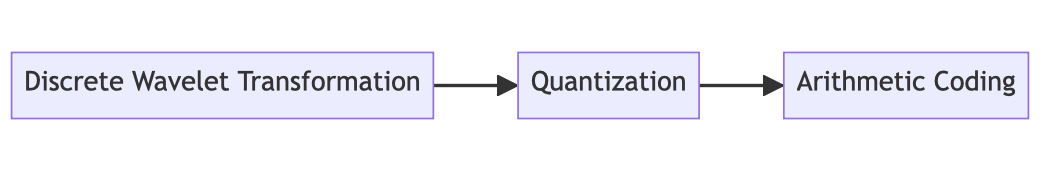
\includegraphics[width=\textwidth]{ct.png}
    \caption[short]{Схема сжатия компоненты}
  \end{figure}

  \paragraph{Discrete Wavelet Transformation}\mbox{}\\
  Над каждой компонентой выполняется двумерное дискретное вейвлет преобра-зование.
  Данная процедура также может быть обратимой (5/3) и необратимой (9/7).

  Суть двемерного вейвлет преобразования - сначала применить стандарт-ное
  одномерное вейвлет преобразование на все строки, затем на все столбцы
  и разбить полученную матрицу на 4 матрицы, каждая из которых описывает свой
  sub-band. В зависимости от количества уровней вейвлет преобразования,
  эта процедура может несколько раз рекурсивно применяться на LL sub-band.

  В одномерном случае DWT - обыкновенная фильтрация, позволяющая из
  строки $x$ получить строку $y$:
  \begin{equation}
    y(2n) = \sum_{j = 0}^{N - 1}x(j)\cdot{h_H(j - 2n)}
  \end{equation}
  \begin{equation}
    y(2n + 1) = \sum_{j = 0}^{N - 1}x(j)\cdot{h_L(j - 2n - 1)}
  \end{equation}

  Различием между обратимым и необратимым преобразованием в данном случае
  являются коэффициенты $h_H$ и $h_H$.

  \begin{table}[H]
    \centering
    \begin{tabular}{| c | c | c |}
      \hline
      i & $h_L(i)$ & $h_H(i)$ \\
      \hline
      0 & 1.115087052456994 & 0.6029490182363579 \\
      \hline
      $\pm 1$ &0.5912717631142470 &-0.2668641184428723 \\
      \hline
      $\pm 2$& -0.05754352622849957 &-0.07822326652898785 \\
      \hline
      $\pm 3$ &-0.09127176311424948& 0.01686411844287495 \\
      \hline
      $\pm 4$& 0 &0.02674875741080976 \\ 
      \hline
      другие i & 0 & 0 \\
      \hline
    \end{tabular}
    \caption{Коэффициенты для необратимого 9/7 преобразования}
  \end{table}

  \begin{table}[H]
    \centering
    \begin{tabular}{| c | c | c |}
      \hline
      i & $h_L(i)$ & $h_H(i)$ \\
      \hline
      0 & $\frac{6}{8}$ & 1 \\
      \hline
      $\pm 1$ & $\frac{2}{8}$ & $-\frac{1}{2}$ \\
      \hline
      $\pm 2$& $-\frac{1}{8}$ & 0  \\
      \hline
      другие i & 0 & 0 \\
      \hline
    \end{tabular}
    \caption{Коэффициенты для обратимого 5/3 преобразования}
  \end{table}

  \begin{figure}[H]
    \centering
    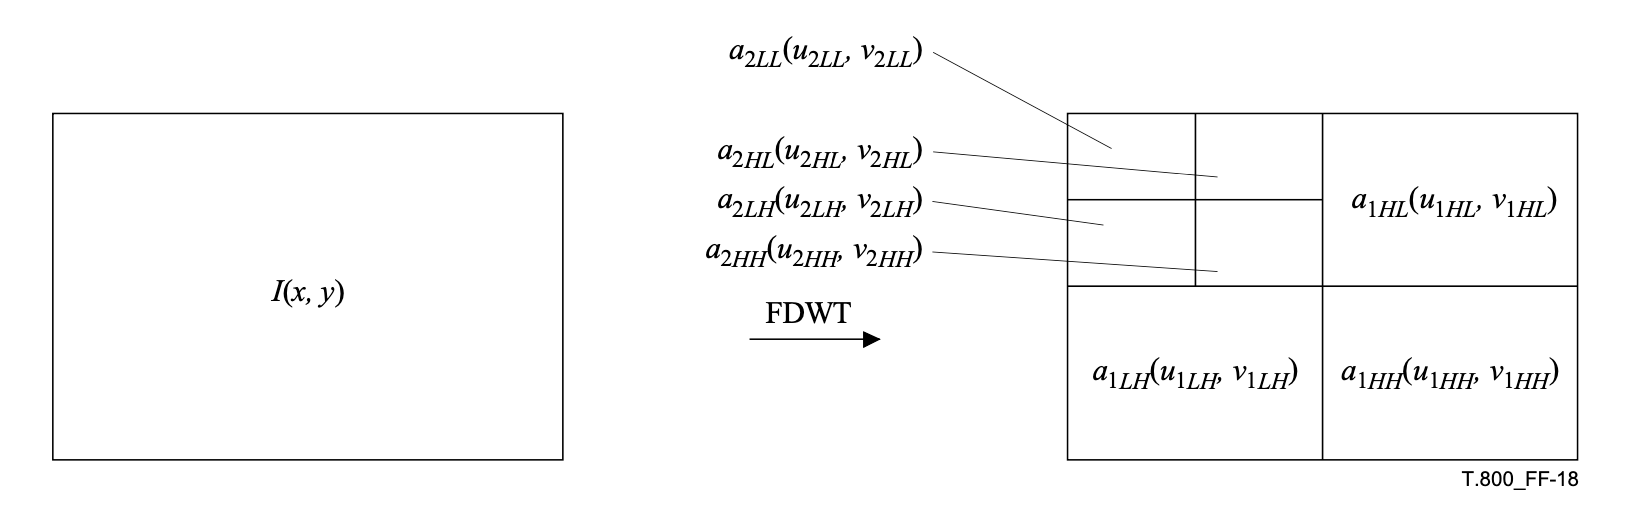
\includegraphics[width=\textwidth]{dwt}
    \caption{Общая схема DWT}
  \end{figure}

  \paragraph{Quantization}\mbox{}\\
  Квантования является опциональным, его основная задача - понижение битнос-ти.
  Также может быть обратимым и необратимым, применяется для уменьше-ния размера
  итогового размера.

  В данной работе не рассматривается в виду своей опциональности и об-щей редкости.

  \paragraph{Arithemic Coding}\mbox{}\\
  Арифметическое ентропийное кодирование - непосредственно процесс сжатия данных.
  Оно учитывает вероятность появления того или иного бита, на основе чего компрессирует данные.

  После вейвлет преобразования получается набор sub-band, каждый из ко-торых
  делиться на блоки (code-block) и кодируется отдельно.

  \begin{figure}[H]
    \centering
    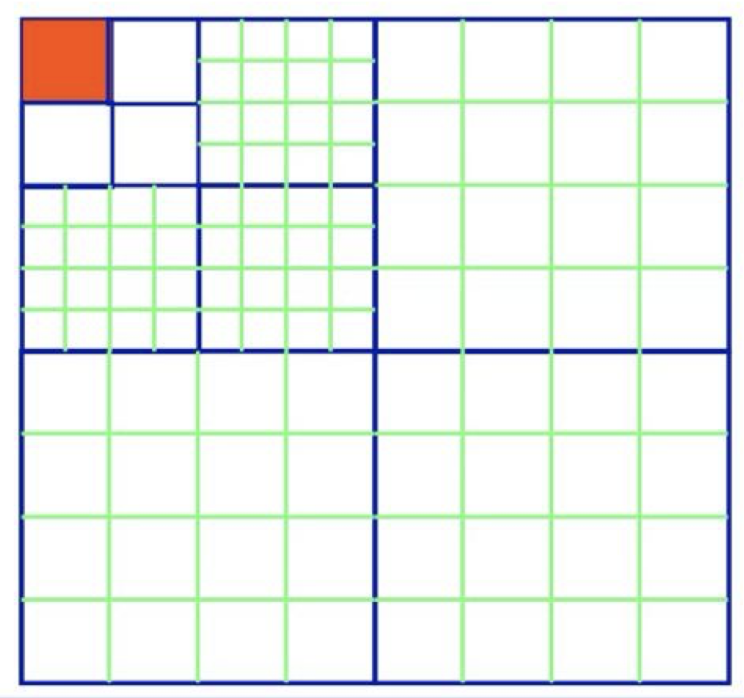
\includegraphics[width=0.5\textwidth]{div.png}
    \caption{Зеленое - границы code-block, синее - границы sub-band}
  \end{figure}

  Размер code-block ограничен сверху 4096 байтами, может иметь любую высоту,
  но обязан быть 16 байт в ширину. Чтение такого блока при кодировании
  происходит столбцами по 4 байта:

  \begin{figure}[H]
    \centering
    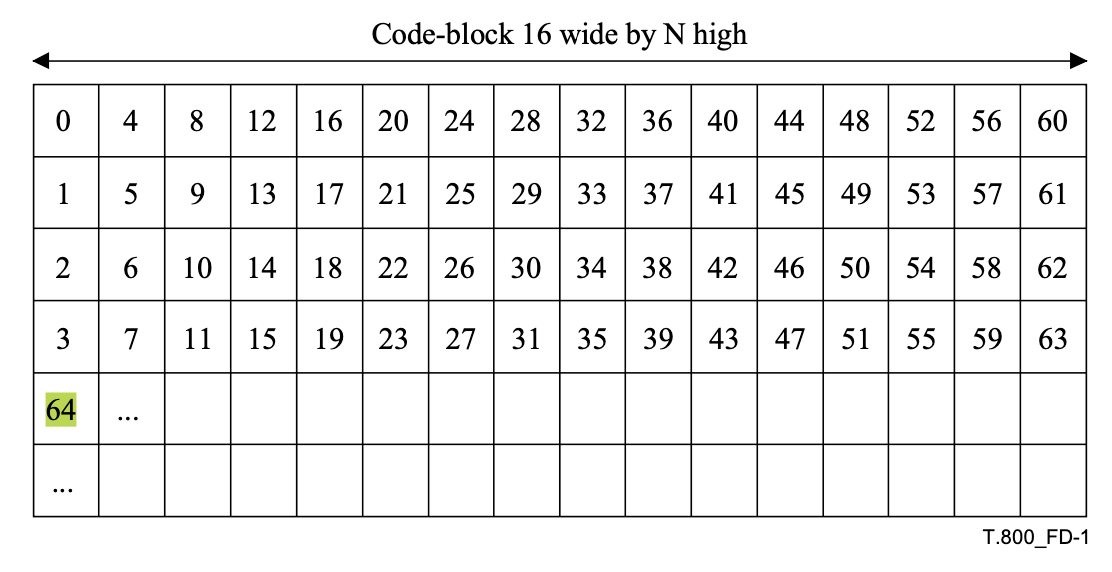
\includegraphics[width=\textwidth]{cb}
    \caption{Порядок чтения code-block}
  \end{figure}

  \subsection{Внутреннее устройство файла}

  Файл в формате JPEG2000 - это набор контейнеров, именуемых боксами. Каждый бокс
  состоит из типа, размера и сырых данных. Сырые данные по типу можно конвертировать
  в реальные значения, описывающие изображение и его свойства.

  Количество боксов в файле не ограничено, начинаться каждый .jp2 дол-жен
  с сигнатурного бокса - набор байт, подтверждающий формат.

  Обязательно должен присутствовать заголовочный контейнер (image he-ader), описывающий размер изображения,
  количество компонент и способ сжа-тия. Также необходим контейнер, описывающий
  используемое цветовое про-странство - он может как указывать на уже известные
  RGB, YCrCb, так и со-держать новую отдельную таблицу цветов в ICC формате.

  Последним обязатеьным боксом является бокс с данными кодстрима. Та-ких боксов
  несколько, их содержимое вместе и явялется сжатым изображением.

  Кодстрим делится на маркеры и маркерные сегменты. Маркеры указыва-ют на начало
  определенной секции - описание кодстрима в целом, описание тайла (часть изображения)
  и сжатые данные.

  \subsection{Выполненные работы}

  В ходе работы была выполнена исследовательская деятельность, нацелен-ная
  на изучение внутреннего устройства формата и принципов работы с ним, а также
  частично реализован функционал, позволяющий кодировть и декодиро-вать изображения в JPEG2000.

  \subsubsection{Boxes reading and writing}

  Присутствует код, который может распарсить файл в формате jpeg2000 на боксы
  и сериализовать их в понятные структуры.

  Процесс десериализации и записи обратно в файл также реализован.

  \subsubsection{DC level shifting}

  Реализован DC level shifting в обе стороны (прямой для кодирования и
  обратный для декодирования) над RGB цветами:

  \begin{code}
    \begin{minted}{c++}
TRGB TJP2Coder::ApplyDCLevelShifting(const TRGB& src) const {
  ui32 deltaR = (RDepth_ & 0x80)? 0 : std::pow(2, RDepth_);
  ui32 deltaG = (GDepth_ & 0x80)? 0 : std::pow(2, GDepth_);
  ui32 deltaB = (BDepth_ & 0x80)? 0 : std::pow(2, BDepth_);
  return TRGB {
    .R = src.R - deltaR,
    .G = src.G - deltaG,
    .B = src.B - deltaB
  };
};
    \end{minted}
    \captionof{listing}{Forward DC level shifting}
  \end{code}

  \begin{code}
    \begin{minted}{c++}
auto TJP2Coder::ApplyInverseDCLevelShifting(
  const TRGB& src
) const -> TRGB {
  ui32 deltaR = (RDepth_ & 0x80)? 0 : std::pow(2, RDepth_);
  ui32 deltaG = (GDepth_ & 0x80)? 0 : std::pow(2, GDepth_);
  ui32 deltaB = (BDepth_ & 0x80)? 0 : std::pow(2, BDepth_);
  return TRGB {
      .R = src.R + deltaR,
      .G = src.G + deltaG,
      .B = src.B + deltaB
  };
};
    \end{minted}
    \captionof{listing}{Inverse DC level shifting}
  \end{code}


  \subsubsection{Multicomponent transformation}

  Описан переход вида $RGB \leftrightarrow YUV$ без потерь:\\

  \begin{code}
    \begin{minted}{c++}
    auto MapToYUV(const TRGB& source) -> TYUV {
        i32 tmp = 0;
        tmp += source.R;
        tmp += source.G;
        tmp += source.G;
        tmp += source.B;
    
        return TYUV {
            .Y = tmp / 4,
            .U = source.B - source.G,
            .V = source.R - source.G
        };
    }
    
    auto MapToRGB(const TYUV& source) -> TRGB {
        i32 temp = 0;
        temp += source.U;
        temp += source.V;
        i32 g = source.Y - temp / 4;
    
        return TRGB {
            .R = source.V + g,
            .G = g,
            .B = source.U + g
        };
    };
    \end{minted}
    \captionof{listing}{Multicomponent transformation}
  \end{code}

  \subsubsection{Discrete wavelet transformation}

  Реализовано прямой и обратное дискретной вейвлет преобразование
  над двумерными массивами:

  \begin{code}
    \begin{minted}{c++}
auto downDiv(i32 a, i32 b) -> i32 {
    if (a >= 0) {
        return a / b;
    } else {
        if (a % b == 0) {
            return a / b;
        } else {
            return a / b - 1;
        }
    }
}

auto upDiv(i32 a, i32 b) -> i32 {
    if (a % b > 0) {
        return a / b + 1;
    } else {
        return a / b;
    }
}

auto Do53DWT(const std::vector<i32>& src) -> std::vector<i32> {
    auto x = [&] (i32 i) {
        if (i < 0) {
            return src.at(-i);
        } else if (i >= src.size()) {
            return src.at(2 * src.size() - i - 2);
        } else {
            return src.at(i);
        }
    };

    std::function<i32(i32)> y = [&] (i32 i) {
        if (i % 2 == 0) {
            return x(i) + downDiv(y(i - 1) + y(i + 1) + 2, 4);
        } else {
            return x(i) - downDiv(x(i - 1) + x(i + 1), 2);
        }
    };
    
    std::vector<i32> result;
    result.reserve(src.size());

    for (i32 i {0}; i < src.size(); i++) {
        result.push_back(y(i));
    }

    return result;
}

auto Transpone(const std::vector<std::vector<i32>>& src) -> std::vector<std::vector<i32>> {
    std::vector<std::vector<i32>> result;

    for (ui64 i {0}; i < src.at(0).size(); i++) {
        std::vector<i32> newRow;
        for (ui64 j {0}; j < src.size(); j++) {
            newRow.push_back(src.at(j).at(i));
        }
        result.push_back(newRow);
    }

    return result;
}


auto BaseMatrixDWT(const std::vector<std::vector<i32>>& src) -> std::vector<std::vector<i32>> {
    std::vector<std::vector<i32>> temp;

    for (ui64 i {0}; i < src.at(0).size(); i++) {
        std::vector<i32> column;
        column.reserve(src.size());

        for (const auto& row : src) {
            column.push_back(row.at(i));
        }

        temp.push_back(Do53DWT(column));
    }

    temp = Transpone(temp);

    std::vector<std::vector<i32>> result;
    for (const auto& row : temp) {
        result.push_back(Do53DWT(row));
    }
    return result;
}

auto Deinterleave(const std::vector<std::vector<i32>>& src) -> TA {
    ui64 v = src.size(), u = src.at(0).size();

    std::vector<std::vector<i32>> ll;
    for (ui64 vb {0}; vb < upDiv(v, 2); vb++) {
        std::vector<i32> row;
        for (ui64 ub {0}; ub < upDiv(u, 2); ub++) {
            row.push_back(src.at(vb * 2).at(ub * 2));
        }
        ll.push_back(row);
    }

    std::vector<std::vector<i32>> hl;
    for (ui64 vb {0}; vb < upDiv(v, 2); vb++) {
        std::vector<i32> row;
        for (ui64 ub {0}; ub < downDiv(u, 2); ub++) {
            row.push_back(src.at(vb * 2).at(ub * 2 + 1));
        }
        hl.push_back(row);
    }

    std::vector<std::vector<i32>> lh;
    for (ui64 vb {0}; vb < downDiv(v, 2); vb++) {
        std::vector<i32> row;
        for (ui64 ub {0}; ub < upDiv(u, 2); ub++) {
            row.push_back(src.at(vb * 2 + 1).at(2 * ub));
        }
        lh.push_back(row);
    }

    std::vector<std::vector<i32>> hh;
    for (ui64 vb {0}; vb < downDiv(v, 2); vb++) {
        std::vector<i32> row;
        for (ui64 ub {0}; ub < downDiv(u, 2); ub++) {
            row.push_back(src.at(vb * 2 + 1).at(ub * 2 + 1));
        }
        hh.push_back(row);
    }

    return TA { .LL = ll, .HL = hl, .LH = lh, .HH = hh};
}


auto Union(const TA& ta) -> std::vector<std::vector<i32>> {
    std::vector<std::vector<i32>> result;

    for (ui64 i {0}; i < ta.LL.size(); i++) {
        std::vector<i32> row;
        for (auto e : ta.LL.at(i)) {
            row.push_back(e);
        }
        for (auto e : ta.HL.at(i)) {
            row.push_back(e);
        }
        result.push_back(row);
    }

    for (ui64 i {0}; i < ta.HH.size(); i++) {
        std::vector<i32> row;
        for (auto e : ta.LH.at(i)) {
            row.push_back(e);
        }
        for (auto e : ta.HH.at(i)) {
            row.push_back(e);
        }
        result.push_back(row);
    }

    return result;
}

auto Do53DWT(
  const std::vector<std::vector<i32>>& src,
  ui32 levels
) -> std::vector<std::vector<i32>> {
    std::vector<TA> result;
    result.push_back(TA { .LL = src, .HL = {}, .LH = {}, .HH = {} });

    for (ui64 i {1}; i <= levels; i++) {
        result.push_back(Deinterleave(
          BaseMatrixDWT(result.at(i - 1).LL)));
    }

    std::vector<std::vector<i32>> combined = result.back().LL;

    for (ui64 i {levels}; i > 0; i--) {
        TA current = result.at(i);
        combined = Union(TA { .LL = combined,
          .HL = current.HL, .LH = current.LH,
            .HH = current.HH });
    }

    return combined;
}
    \end{minted}
    \captionof{listing}{Forward DWT}
  \end{code}

  \subsubsection{Codestream reading and writing}

  Реализовано чтение и запись основных маркеров для понимания и работы с codestream.

  \subsubsection{Что не удалось}

  Не удалось выработать контекст для арифметического кодирования, в
  связи с этим нет полноценной реализации кодека для JPEG2000.

  \newpage
  \section{Заключение}

  В ходе данной работы не удалось полностью реализовать стандарт, но
  были реализованы некоторые его составные части, на основе которых, 
  с допол-нением в виде арифметического кодирования, можно выполнить
  полноценный кодек.

  Были рассмотрены различные формы дискретного вейвлет преобразова-ния,
  а также методы перехода между различными цветовыми пространствами.

  \newpage
  \section{Список использованных источников}

  \begin{thebibliography}{9}
    \bibitem{texbook}
    Skodras, A., Christopoulos, C. and Ebrahimi, T., 2001. The JPEG 2000 still image compression standard. IEEE Signal processing magazine, 18(5), pp.36-58.

    \bibitem{texbook}
    Schelkens, P., Skodras, A. and Ebrahimi, T. eds., 2009. The JPEG 2000 suite. John Wiley and Sons.

    \bibitem{texboox}
    Information technology – JPEG 2000 image coding system: Core coding system - ITU-T -2015
  
    \bibitem{textbook}
    Taubman, D.S. and Marcellin, M.W., 2002. JPEG2000: Standard for interactive imaging. Proceedings of the IEEE, 90(8), pp.1336-1357.
  \end{thebibliography}

\end{document}

